\chapter{Теоретико-аналитическая часть}

  \section{Постановка задачи}

    Исследовать возможность использования семантико-синтаксического
    анализатора Compreno в качестве источника высокоуровневых признаков для задачи
    NER на корпусе CoNLL 2003 в рамках нейросетевого подхода.

  \section{Обзор литературы}

    Победители соревнования по NER CoNLL 2003 \citep{florian2003named}, получившие 88.76\% F1,
    представили систему использующую комбинацию различных алгоритмов машинного обучения.
    В качестве признаков был использован их собственный, вручную составленный газетир,
    POS-теги, CHUNK-теги, суффиксы, префиксы и выход других NER-классификаторов,
    тренированных на внешних данных.

    \citep{collobert2011natural} представили комбинацию сверточной нейронной сети
    с условными случайными полями, получившую 89.59\% F1 на корпусе CoNLL 2003.
    Их нейросетевая архитектура не зависит от задачи и используется как для NER, так и для
    частеречной разметки (part-of-speech tagging), поиска синтаксически связанных групп
    соседних слов (chunking), установления семантических ролей (semantic role labelling).
    Для задачи NER они использовали три типа признаков - векторное представление слова,
    капитализацию и небольшой газетир, включенный в соревнование CoNLL 2003.

    \citep{chiu2015named} представили комбинацию сверточных сетей, рекуррентных сетей
    и условных случайных полей.
    Они использовали такие же признаки как у \citep{collobert2011natural}, дополнительный, вручную сформированный
    газетир на основе DBpedia и обучались на
    train+dev\footnote{Объединенная обучающая и валидационная выборки} выборке CoNLL 2003.
    У них получилось 91.62\% F1. Кроме корпуса CoNLL 2003 они тестировали архитектуру
    на более крупном англоязычном корпусе OntoNotes 5.0. На нем они получили
    state-of-the-art результат 86.28\%.

    \citep{DBLP:journals/corr/YangSC16} представили глубокую иерархическую рекуррентную нейросетевую
    архитектуру с условными случайными полями для разметки последовательностей.
    Они использовали такие же признаки как у \citep{collobert2011natural}.
    Кроме англоязычного корпуса CoNLL 2003, где они получили state-of-the-art 90.94\% F1 при обучении
    только на обучающей выборке (train set), они тестировали работу нейросети на CoNLL 2002 Dutch NER и CoNLL 2003 Spanish NER.
    На этих корпусах они улучшили предыдущий state-of-the-art результат:
    82.82\% до 85.19\% на CoNLL 2002 Dutch NER и 85.75\% до 85.77\% на CoNLL 2003 Spanish NER.

    Современные работы используют векторное представление слов
    и условные случайные поля в своих моделях. Из сторонних признаков применяют
    только газетиры. В работах \citep{xu2014rc, bian2014knowledge} описано применение дополнительных признаков для
    слов (морфологических, синтаксических, семантических) для создания более
    совершенных векторных представлений.
    Такие векторные представления помогают повысить оценку качества в
    прикладных задачах \citep{xu2014rc}.

  \section{Обзор методов решения задачи}

    \subsection{Условные случайные поля}

      Условные случайные поля (conditional random fields) - это семейство дискриминативных
      вероятностных графических моделей, которые применяются для решения задачи обучения с учителем.
      Обычно их используют для задач, связанных с разметкой последовательностей, например,
      распознавание именованных сущностей, частеречной разметки.

      \textbf{Плюсы:}
        \begin{itemize}
          \item{показывают хороший результат для задачи NER на CoNLL 2003 (88-89\%).}
        \end{itemize}

      \textbf{Минусы:}
        \begin{itemize}
          \item{необходимо заниматься инженерией признаков,}
          \item{долгое время обучения модели.}
        \end{itemize}

      Примеры библиотек: http://www.chokkan.org/software/crfsuite/

      \begin{figure}
      \centering
      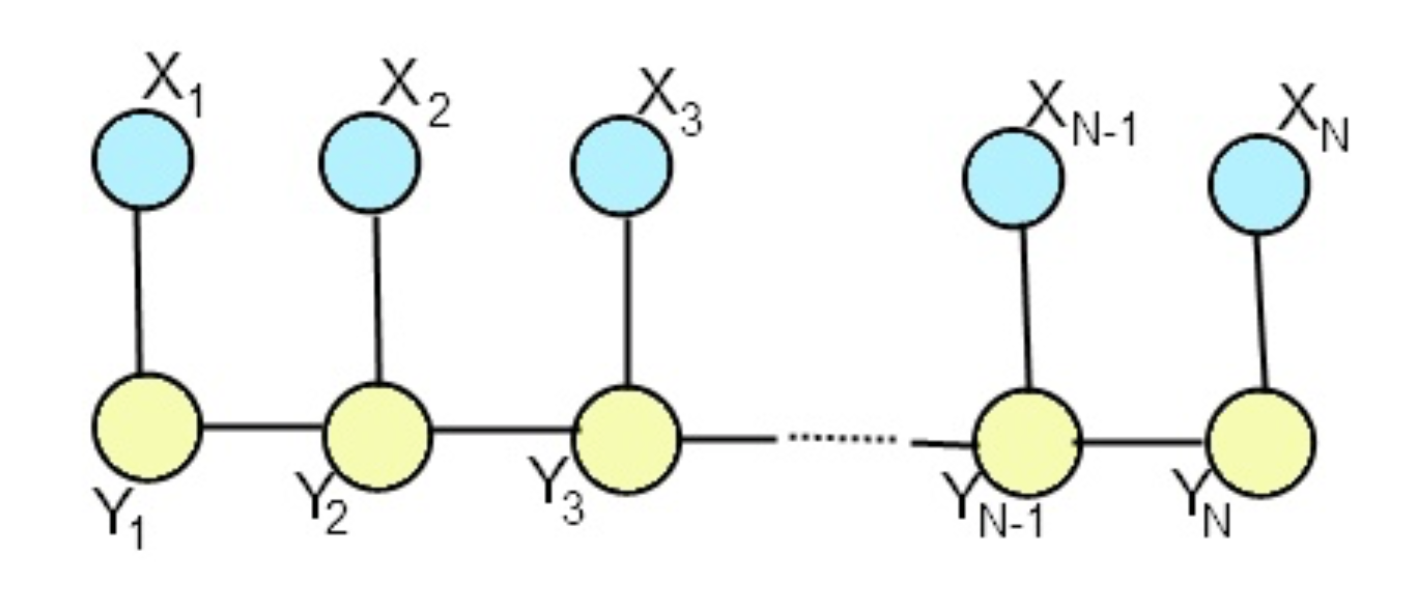
\includegraphics[width=\textwidth]{figures/crf.png}
      \caption{Условные случайные поля в виде линейной цепи}
      \label{fig:crf}
      \end{figure}

    \subsection{Нейронные сети}
      Искусственные нейронные сети - это семейство дискриминативных моделей, которые
      имитируют работу биологической нейронной сети. Их применяют для самых разных задач
      машинного обучения, начиная кластеризацией и заканчивая обучением с подкреплением.

      \textbf{Плюсы:}
        \begin{itemize}
          \item показывают достаточно хороший результат для задачи NER на CoNLL 2003 (87-88\%),
          \item быстро обучаются,
          \item расширяемы, если использовать специальные фреймворки,
          \item судя по опыту, точность растет с увеличением набора данных,
          \item не нужно вручную отбирать и создавать признаки.
        \end{itemize}

      \textbf{Минусы:}
        \begin{itemize}
          \item нужен графический процессор,
          \item тяжело объяснить на основе чего модель приняла определенное решение.
        \end{itemize}

      Примеры библиотек: http://torch.ch, https://www.tensorflow.org
      \newpage
      \begin{figure}
      \centering
      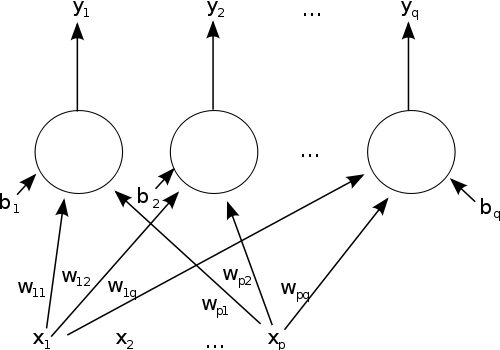
\includegraphics[width=\textwidth]{figures/ann.png}
      \caption{Пример искусственной нейронной сети}
      \label{fig:ann}
      \end{figure}

    \subsection{Комбинация нейронных сетей и условных случайных полей}
      Комбинацию нейронных сетей и условных случайных полей получают путем модификации
      функции потерь нейронной сети.

      \textbf{Плюсы:}
        \begin{itemize}
          \item показывают лучший результат для задачи NER на CoNLL 2003 (89-90\%),
          \item такие же как у нейросетей.
        \end{itemize}

      \textbf{Минусы:}
        \begin{itemize}
          \item такая комбинация тяжела в реализации с нуля,
          \item не поддерживаются существующими фреймворками,
          \item такие же как у нейросетей.
        \end{itemize}
      Примеры библиотек: нет.
      \newpage

      \begin{figure}
      \centering
      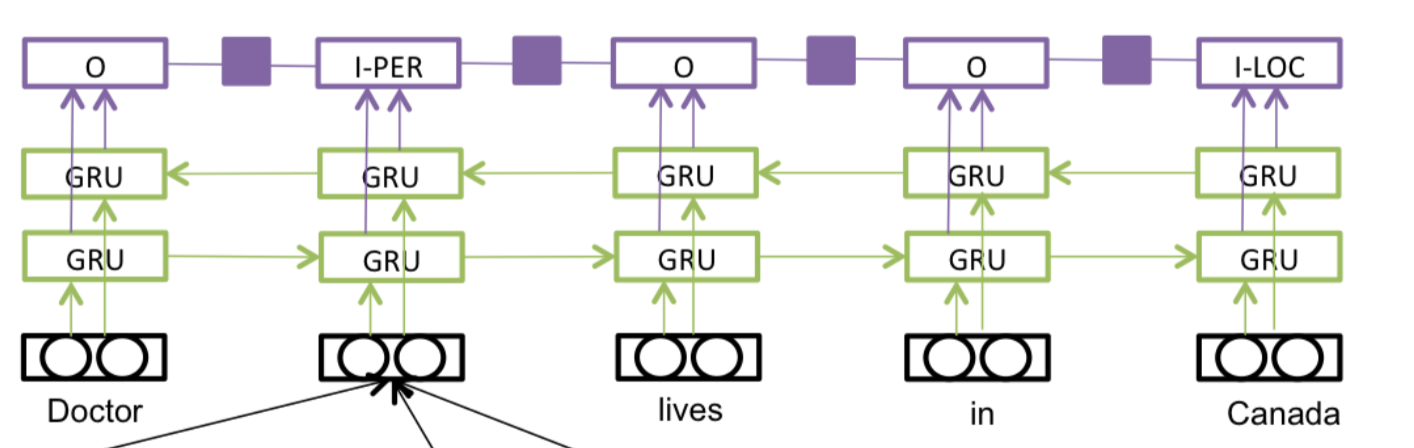
\includegraphics[width=\textwidth]{figures/nn+crf.png}
      \caption{Пример комбинации нейронной сети и условных случайных полей из \citep{DBLP:journals/corr/YangSC16}}
      \label{fig:rnncrf}
      \end{figure}

    \subsection{Выбор метода решения задачи}

      Лучший результат для задачи NER на CoNLL 2003 показывает комбинация нейросети и
      условных случайных полей. Они довольно сложны в реализации с нуля, т.к. не поддерживаются
      существующими фреймворками.

      Условные случайные поля сами по себе показывают неплохой
      результат, но долго обучаются и требуют сложную инженерию признаков.

      Нейронные сети показывают достаточно хороший результат, быстро обучаются,
      расширяемы и
      имеют различные Open Source библиотеки, поддерживаемые сообществом и крупными
      компаниями, такими как Facebook, Google, Yandex.
      Исходя из цели работы был выбран нейросетевой подход. В перспективе в него
      можно внедрить условные случайные поля для получения state-of-the-art результата.

  \section{Синтактико-семантические признаки}
    Существует много инструментов для получения дополнительных признаков для слова.
    Для извлечения синтаксических признаков часто используют MaltParser \citep{nivre2006maltparser}.
    Для получения семантических признаков применяют BabelNet \citep{navigli2010babelnet}.

    В данной работе для получения синтактико-семантических признаков используется Compreno.
    Вершины синтактико-семантического дерева Compreno кодировались бинарным представлением
    и соотносились с токенами исходного
    текста\footnote{Почти для всех токенов в соответствующем дереве нашлась соответствующая вершина.
    Токены для которых не была найдена вершина, кодировались специальным признаком 83951},
    тем самым наделяя их синтактико-се\-ман\-ти\-ческими признаками.
    Размерность пространства синтактико-се\-ман\-ти\-ческих признаков получилась равной 83950.

    Плотные вектора большой размерности сильно замедляют процесс оптимизации и для хорошего
    обучения требуется много данных и вычислительных ресурсов.
    В таких случаях часто применяют методы для уменьшения размерности,
    например сингулярное разложение или автоэнкодеры. Минусом таких методов является потеря информации
    после сжатия.

    Если же вектора большой размерности разреженные, то используют специальные методы для
    работы с такими данными \citep{davissurvey}.

    В данной работе предлагается 2 способа внедрения синтактико-семантических признаков:
    \begin{itemize}
      \item сжать синтактико-семантические вектора с помощью сингулярного разложения (SVD) и добавить
      как еще один Lookup Table в сверточную нейронную сеть;
      \item добавить еще одну нейронную сеть для синтактико-семантических признаков и оптимизировать
      её вместе со сверточной нейронной сетью.
    \end{itemize}
